\subsection*{\textbf{\RQsix}}

We report the results of $RQ6$ in two subsections. First, we report on the release processes of our participants' projects in general (i.e., not considering influences of CI yet). This is important to obtain an overview of the variety of release processes in our data and will provide us with more context when interpreting the influence of CI on release processes. 
Afterward, we show the perceived influence of CI on the release processes of our participants' projects.

\vspace{2mm}
\noindent\textbf{Release processes in general.}
\vspace{2mm}

According to our participants, the release process of their project are \textit{goal oriented},\textsuperscript{(97)} \textit{maintainer oriented},\textsuperscript{(18)} follow a specific \textit{release strategy},\textsuperscript{(94)} such as \textit{continuous delivery},\textsuperscript{(28)} and are driven by \textit{business}\textsuperscript{(18)} and \textit{user demand}.\textsuperscript{(7)} In addition, some participants perceive an \textit{ad hoc}\textsuperscript{(7)} approach to the release process of their project. Table~\ref{tab:freq_citations_project_releasing_process} shows the citation frequency of each theme and code related to the release process of projects.

% Table generated by Excel2LaTeX from sheet 'Sheet3'
\begin{table}
	\centering
	\caption{Frequency of themes and codes as captured from our participants' responses.}
	\begin{tabular}{p{8.915em}rrc}
		\hline
		\multirow{2}[4]{*}{\textbf{Theme}} & \multicolumn{1}{c}{\multirow{2}[4]{*}{\textbf{Code}}} & \multicolumn{2}{p{9.33em}}{\textbf{Frequency}} \bigstrut\\
		\cline{3-4}    \multicolumn{1}{c}{} &       & \multicolumn{1}{p{4.665em}}{\textbf{Frequency per Code}} & \multicolumn{1}{p{4.665em}}{\textbf{Frequency per Theme}} \bigstrut\\
		\hline
		\multirow{7}[14]{*}{\textbf{Goal oriented}} & \multicolumn{1}{p{11.915em}}{Code stability} & \multicolumn{1}{c}{28} & \multirow{7}[14]{*}{97} \bigstrut\\
		\cline{2-3}    \multicolumn{1}{c}{} & \multicolumn{1}{p{11.915em}}{New feature} & \multicolumn{1}{c}{22} &  \bigstrut\\
		\cline{2-3}    \multicolumn{1}{c}{} & \multicolumn{1}{p{11.915em}}{Tested code} & \multicolumn{1}{c}{13} &  \bigstrut\\
		\cline{2-3}    \multicolumn{1}{c}{} & \multicolumn{1}{p{11.915em}}{Feature completeness} & \multicolumn{1}{c}{10} &  \bigstrut\\
		\cline{2-3}    \multicolumn{1}{c}{} & \multicolumn{1}{p{11.915em}}{Enough content} & \multicolumn{1}{c}{10} &  \bigstrut\\
		\cline{2-3}    \multicolumn{1}{c}{} & \multicolumn{1}{p{11.915em}}{Project roadmap} & \multicolumn{1}{c}{7} &  \bigstrut\\
		\cline{2-3}    \multicolumn{1}{c}{} & \multicolumn{1}{p{11.915em}}{Project milestone} & \multicolumn{1}{c}{7} &  \bigstrut\\
		\hline
		\multirow{5}[10]{*}{\textbf{Release strategy}} & \multicolumn{1}{p{11.915em}}{Fixed periods} & \multicolumn{1}{c}{49} & \multirow{5}[10]{*}{94} \bigstrut\\
		\cline{2-3}    \multicolumn{1}{c}{} & \multicolumn{1}{p{11.915em}}{Continuous delivery} & \multicolumn{1}{c}{28} &  \bigstrut\\
		\cline{2-3}    \multicolumn{1}{c}{} & \multicolumn{1}{p{11.915em}}{Release schedule} & \multicolumn{1}{c}{10} &  \bigstrut\\
		\cline{2-3}    \multicolumn{1}{c}{} & \multicolumn{1}{p{11.915em}}{Release early, release often practice} & \multicolumn{1}{c}{4} &  \bigstrut\\
		\cline{2-3}    \multicolumn{1}{c}{} & \multicolumn{1}{p{11.915em}}{Time-based release} & \multicolumn{1}{c}{3} &  \bigstrut\\
		\hline
		\textbf{Maintainer oriented} &       &       & 18 \bigstrut\\
		\hline
		\textbf{Business-driven} &       &       & 18 \bigstrut\\
		\hline
		\textbf{User demand} &       &       & 7 \bigstrut\\
		\hline
		\textbf{Ad hoc} &       &       & 7 \bigstrut\\
		\hline
	\end{tabular}%
	\label{tab:freq_citations_project_releasing_process}%
\end{table}%

\textit{Goal oriented}\textsuperscript{(97)} is the theme that emerged the most when it comes to the release process of our participants' projects. An example of a goal that projects strive to achieve is \textit{code stability}.\textsuperscript{(28)} As C370 explains, their project creates a release \textit{``when the API is stable and extensively tested.''} Other participants also explain that their projects produce a release when a desired \textit{new feature} has been developed,\textsuperscript{(22)} the \textit{code has been tested},\textsuperscript{(13)} or \textit{enough content}\textsuperscript{(10)} has been developed to launch a new version of the software. For example, C178 explains that \textit{``it [the release] is usually done when enough new features and patches have been made.''} 
Therefore, we observe that some participants perceive that their projects adopt a more traditional release strategy (as opposed to rapid releases~\citep{Da_Costa2016-cb}) to deliver new versions of their project. This strategy may also be called \textit{feature-based releases}, where a project launches a new release when a set of bug fixes and new features are ready~\citep{michlmayr2015and}. However, {\em feature-based releases} may not be ideal in a volunteer-based open-source project. For example, there is a risk that projects have an unpredictable release schedule, where releases may take a long time to be launched or never happen due to certain features never being completed \citep{michlmayr2015and}.

In a different vein, when explaining the release process of certain projects, our participants perceive that they adopt a more modern \textit{release strategy}.\textsuperscript{(94)} For example, in certain projects, there exist \textit{fixed periods}\textsuperscript{(49)} and a predictable \textit{release schedule}\textsuperscript{(10)} for launching new releases. Other projects use \textit{continuous delivery}\textsuperscript{(28)} or follow the \textit{release early, release often}\textsuperscript{(4)} practice. C032 explains that in the \textit{saltstack/salt} project there is a \textit{fixed period}\textsuperscript{(49)} for its releases, \textit{``feature release every 6 months, bug fix releases when necessary"}. 
Practices such as \textit{release early, release often} are well established in open source development, which leads to benefits related to quality and consistency as errors can be detected sooner \citep{fitzgerald2017continuous}.   

Some participants have recurrently mentioned that the release process of their project is \textit{maintainer oriented},\textsuperscript{(18)} \textit{business driven},\textsuperscript{(18)} or dependent on the \textit{user demand}.\textsuperscript{(7)} We also observe seven citations that state that the process is not clearly defined or is \textit{ad hoc}.\textsuperscript{(7)} For instance, C444 explains that the \textit{bokeh/bokeh} project \textit{``is volunteer based, so [the release is launched] when we can and think it's reasonable.''} C117 also states that the \textit{fog/fog} project produces its release \textit{``when the maintainer decided it was time to do so.''} Additionally, C003 states that the act of launching a release in \textit{grails/grails-core} \textit{``is a decision between business and the development team.''} The release process may also depend on the outreach of the release. For instance, C302 explains that an important factor to produce a release in \textit{boto/boto} is \textit{``when [they] need a wider audience.''}

\begin{center}
	\begin{tabular}{|p{.95\columnwidth}|}
		\hline
	\textit{Our participants perceive different release strategies for their project. Some projects follow a feature-based release strategy, whereas others adopt a time-based release approach (e.g., release based on business needs or user demands).} \\
		\hline
	\end{tabular}
\end{center}

\vspace{2mm}
\noindent\textbf{The influence of CI on release processes.}
\vspace{2mm}

\noindent\textbf{52.3\% (\nicefrac{168}{321})  of the developers perceive an increase in release frequency after the adoption of CI.} 15.9\%  (\nicefrac{51}{321})  of the developers do not perceive any influence from CI on release processes. Also, 3.4\% (\nicefrac{11}{321}) agree that CI leads to a decrease in the number of releases while 28.3\%  (\nicefrac{91}{321}) refrain from stating an opinion (i.e., the participants do not know of or are unsure about an influence of CI on release processes, see Figure \ref{fig:perc_perceived_impact_of_ci_releasing_process}).

\begin{figure}[H]
	\centering
	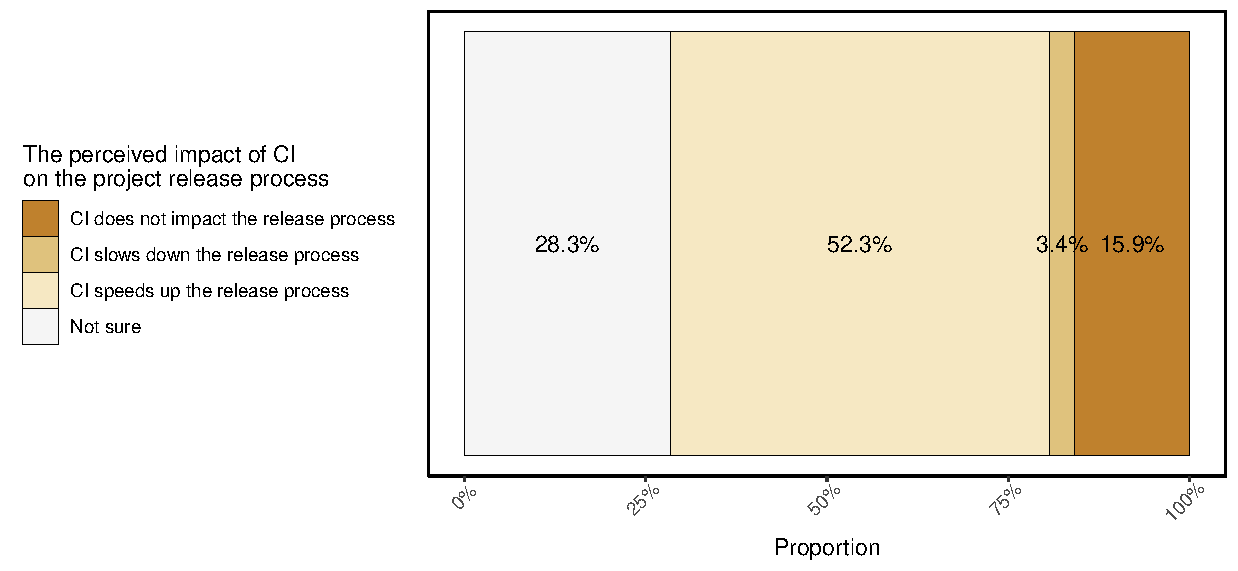
\includegraphics[ width=12cm]{percentage_perceived_impact_of_CI_releasing_process.pdf}
	% figure caption is below the figure
	\caption{Percentage of the perceived influence of CI on release processes (\textit{Question \#18}).}
	\label{fig:perc_perceived_impact_of_ci_releasing_process}       % Give a unique label
\end{figure}

\noindent\textbf{CI increases the release frequency by improving \textit{automation},\textsuperscript{(59)} \textit{project stability},\textsuperscript{(47)} and \textit{release characteristics}.\textsuperscript{(13)}} Table \ref{tab:CI_impacts_on_the_releasing_process} shows the frequency of citations identified for each theme related to the use of CI that may impact the project release process. Each theme is described in the following.

% Table generated by Excel2LaTeX from sheet 'Q18'
\begin{table}
	\centering
	\caption{Frequency of citations for each theme and code related to CI that might impact the project release process.}
	\begin{tabular}{cp{9.25em}cc}
		\hline
		\multicolumn{1}{c}{\multirow{2}[4]{*}{\textbf{Theme}}} & \multirow{2}[4]{*}{\textbf{Code}} & \multicolumn{2}{p{10em}}{\textbf{Frequency}} \bigstrut\\
		\cline{3-4}          & \multicolumn{1}{c}{} & \multicolumn{1}{p{5em}}{\textbf{Frequency per code}} & \multicolumn{1}{p{5em}}{\textbf{Frequency per theme}} \bigstrut\\
		\hline
		\multicolumn{1}{c}{\multirow{6}[12]{*}{\textbf{Automation}}} & Automated testing & 24    & \multirow{6}[12]{*}{59} \bigstrut\\
		\cline{2-3}          & Release automation & 17    &  \bigstrut\\
		\cline{2-3}          & Earlier feedback & 11    &  \bigstrut\\
		\cline{2-3}          & Easier to produce a release & 3     &  \bigstrut\\
		\cline{2-3}          & Automated building & 2     &  \bigstrut\\
		\cline{2-3}          & Earlier integration & 2     &  \bigstrut\\
		\hline
		\multicolumn{1}{c}{\multirow{4}[8]{*}{\textbf{Project Stability}}} & Confidence & 35    & \multirow{4}[8]{*}{47} \bigstrut\\
		\cline{2-3}          & Code stability & 6     &  \bigstrut\\
		\cline{2-3}          & Releasable master & 3     &  \bigstrut\\
		\cline{2-3}          & Less regressions & 3     &  \bigstrut\\
		\hline
		\multicolumn{1}{c}{\multirow{4}[8]{*}{\textbf{Release characteristics}}} & Minor releases & 5     & \multirow{4}[8]{*}{13} \bigstrut\\
		\cline{2-3}          & Smaller releases & 3     &  \bigstrut\\
		\cline{2-3}          & Bug fix releases & 3     &  \bigstrut\\
		\cline{2-3}          & Security releases & 2     &  \bigstrut\\
		\hline
	\end{tabular}%
	\label{tab:CI_impacts_on_the_releasing_process}%
\end{table}%

\vspace{1mm}
\noindent\textbf{Automation.\textsuperscript{(59)}} In the previous subsection, we identified {\em automation} as one of the themes that may quicken the time to deliver merged PRs. In this subsection, we identify that 59 of our participants draw a relationship between {\em automation} improvements brought by CI and the increase in release frequency. For example, \textit{automated tests}\textsuperscript{(24)} and \textit{release automation}\textsuperscript{(17)} are frequently cited when participants explain the increase in release frequency. As explained by C070, \textit{``The testing becomes much simpler and automated, thus it takes less time to validate a release.''} C79 complements the previous answer when they state that \textit{``CI helps with automated tests, so we can merge and release faster.''} Furthermore, when discussing the benefits of CI in relation to release automation, C252 states: \textit{``we can do release often with CI. It's automated.''} 
CI is seen as a continuous deployment enabler, as explained by C327: \textit{``with CI, you can increase the frequency because CI can also deploy automatically.''} 

\vspace{1mm}
\noindent\textbf{Project stability.\textsuperscript{(47)}} The release process of projects is impacted by project stability. The most cited code related to project stability is \textit{confidence}.\textsuperscript{(35)} For instance, C084 states that \textit{``with the confidence gained from CI jobs, maintainers can reduce their time with testing tasks and focus on releases/new features.''}  C056 also states that \textit{``CI allows to keep a releasable master-branch at all times and allows external parties to rely on the quality of master.''} The feedback from our participants reveals that \textit{code stability}\textsuperscript{(35)} allows releases to be prepared more easily. 
C331 expresses that, because CI reduces the number of blocking issues, creating a release becomes easier: \textit{``it [CI] in general contributes to fewer bugs so there are less blocking issues so it is easier to follow a release schedule.''}

\vspace{1mm}
\noindent\textbf{Release characteristics.\textsuperscript{(13)}} The adoption of CI is also mentioned to have changed certain characteristics of releases, which might lead to a higher frequency of releases over time. Several participants perceive that the adoption of CI started a trend of \textit{smaller}\textsuperscript{(3)} and \textit{minor releases}.\textsuperscript{(5)} Participant C203 from \textit{chef/chef} explains the following: \textit{``Yes it [CI] made releases and deployments much more frequent. It removed a lot of manual testing effort and validation. It also changed the culture of the team in such a way that people delivered changes in a smaller and more incremental way.''} Additionally,  participants also perceived an increase in \textit{bugfix}\textsuperscript{(3)} and \textit{security fix}\textsuperscript{(2)} releases. 

15.9\% (\nicefrac{51}{321})  of participants do not perceive any influence from CI on the release process of their projects. According to such participants, the release frequency is \textit{maintainer oriented}\textsuperscript{(2)}, depends strictly on the project \textit{release policy}\textsuperscript{(1)} or depends on the \textit{project maturity}.\textsuperscript{(1)} According to participants, instead of influencing the release frequency, CI influences the \textit{merge time}\textsuperscript{(1)}, \textit{quickens the testing process}\textsuperscript{(1)}, and provides \textit{better quality}\textsuperscript{(5)}. For instance, C317 states that \textit{``CI may help add more features. It should not increase the frequency of releases essentially. It is a matter of policy I think.''} Additionally, C110 expresses: \textit{``It looks like it depends on wish of repository owners and their plan''}. On another note, C169 perceives that the increase in release frequency is a side-effect of the maturation of a project, which can occur due to the adoption of CI: \textit{``Only insofar as adoption of CI indicates the professionalization of a project, which can be correlated with more frequent releases.''} 

Finally, only 3.4\%  (\nicefrac{11}{321}) of participants perceive that CI decreases the release frequency in their projects. According to 11 participants, the decrease in release frequency can be related to the influence of CI on code \textit{stability}\textsuperscript{(2)} and \textit{quality}.\textsuperscript{(2)} For instance, C094 explains that in \textit{ipython/ipython} \textit{``The releases are bit less frequent. The use of CI makes the code more tested and lowers a need for bugfix-minor releases.''} Additionally, C257 declares that \textit{``CI made the number of releases smaller and less frequent, because it helped to catch errors in the code during review. While this made releasing slower, it made the quality of those releases much better.''}  

\begin{center}
\begin{tabular}{|p{.96\columnwidth}|}
    \hline
    \textbf{Summary:}
    \textit{52.3\% (\nicefrac{168}{321})  of participants perceive an increase in the release frequency after the adoption of CI. This increase is related to improvements brought by CI, such as better \textit{automation}, \textit{project stability}, and changes in \textit{release characteristics} (e.g., smaller releases). Furthermore, only 3.4\%  (\nicefrac{11}{321}) of participants agree that CI decreases the release frequency of their projects.} \\
    \textbf{Implications:}
    \textit{Teams planning to improve their release process should consider the adoption of CI, which will not always release more often. However, the automation provided by CI fosters more confidence in releasing the software.}
    \\
    \hline
\end{tabular}
\end{center}